\chapter{Lecture 5 - MATLAB Functions for Root Finding}
\label{ch:lec5n}
\section{Objectives}
The objectives of this lecture are to:
\begin{itemize}
\item Describe the goals for more advanced root-finding algorithms and generally outline how they may be achieved.
\item Discuss MATLAB's built-in function \lstinline[style=myMatlab]{fzero} for finding roots of non-linear functions.
\item Illustrate how to use the advanced features of fzero.
\end{itemize}
\setcounter{lstannotation}{0}

\section{Goals for Advanced Root-Finding Algorithms}

The bisection method that we studied in Lecture 3 is reliable but convergence is slow.  In particular it exhibits linear convergence where:
\begin{equation}
e_{i+1} = \frac{1}{2}e_{i}
\end{equation}
Newton's method, that we learned about in Lecture 4, converges fast when everything works as hoped, but is relatively unreliable.  What we want, of course, is an algorithm that converges \emph{super-linearly} and \emph{almost} never fails.

\section{Regula Falsi Method}
The regula falsi method is a simple alternative to the bisection method that holds the promise (potentially) for faster convergence.  The method starts with a bracket $[a,b]$ like the bisection method but, instead of using the midpoint of the bracket for the next estimate of the solution, the regula falsi method uses the point in $[a,b]$ where the \emph{secant line} between $f(a)$ and $f(b)$ is equal to zero.  A schematic of the first two iterations is illustrated in Figure \ref{fig:lec3n-regula-falsi}.
\begin{marginfigure}
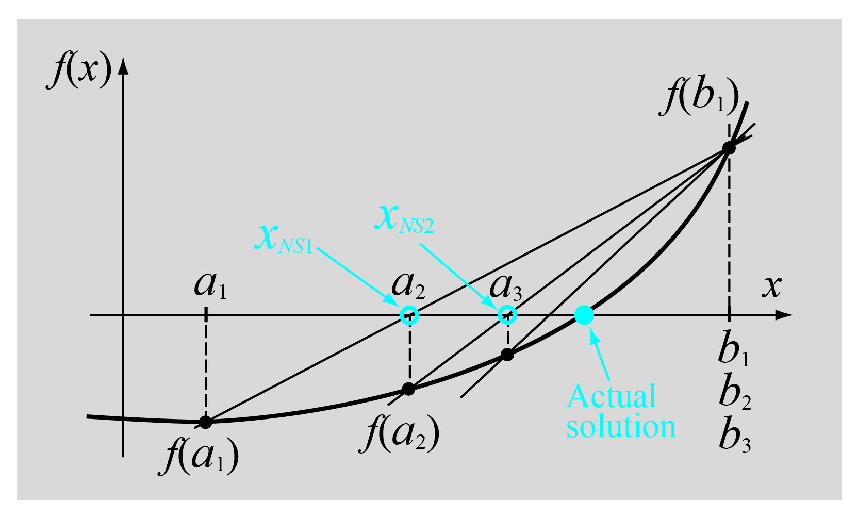
\includegraphics{Chapter3_Fig3_9.eps}
\caption{The first two iterations of the regula falsi method.}
\label{fig:lec3n-regula-falsi}
\end{marginfigure}
The straight line connecting $f(a)$ to $f(b)$ is given by Equation \ref{eq:lec3n-regula-falsi}:
\begin{equation}
y = \frac{f(b) - f(a)}{b-a}(x-b)+f(b)
\label{eq:lec3n-regula-falsi}
\end{equation}
The point where the line intersects the $x$-axis is found by setting $y=0$ and solving for $x$, giving us:
\begin{equation}
x_{\text{NS}} = \frac{a f(b) - b f(a)}{f(b) - f(a)}
\label{eq:lec3n-regula-falsi-xns}
\end{equation}
The algorithm for the regula falsi method is as follows:
\begin{enumerate}
\item Find an interval $[a,b]$ in which a root exists.  One way to find such an interval is to identify an $a$ and $b$ for which $f(a)f(b)<0$.
\item Use Equation \ref{eq:lec3n-regula-falsi-xns} to find the new estimate of the numerical solution.
\item Determine whether the root is in $[a,x_{\text{NS}}]$ or in $[x_{\text{NS}},b]$ using the following method:
\begin{itemize}
\item If $f(a)f(x_{\text{NS}}) < 0$, the root is in $[a,x_{\text{NS}}]$.
\item If $f(x_{\text{NS}})f(b) < 0$, the root is in $[x_{\text{NS}},b]$.
\end{itemize}
\item Select the subinterval that contains the solution---either $[a,x_{\text{NS}}]$ or $[x_{\text{NS}},b]$ as determined in step 3---as the new $a$ and $b$ and return to step 2.
\end{enumerate}
The iteration should be stopped when the estimated error is smaller than the pre-determined tolerance.  Some notes on this method:
\begin{itemize}
\item Like the bisection method, the regula falsi method \emph{will} converge.  One can hope that, given the small added complexity, the rate of convergence would be somewhat faster using the regula falsi method.
\item For a given function, it is typically the case that only one endpoint will ``move towards'' the solution.  Modifications to the algorithm can be made to address this issue.  An example of this, that will be included in the homework assignment, is to combine a step of the bisection method along with the regula falsi method.  This measure helps ensure that the interval around the root is consistently reduced from both directions. 
\item Newton's method, the secant method, and regula falsi method all, in one way or another, use linear interpolation to estimate the location of the root.  We might hope to get a better approximation of the root if we used a higher-order interpolant.\sidenote{This is an idea that we will return to in our lectures on interpolation.} Brent's method combines root-bracketing, secant method, and \emph{inverse quadratic interpolation} methods and is the basis of MATLAB's \lstinline[style=myMatlab]{fzero} function.\cite{forsythe1977computer}
\end{itemize}


\section{MATLAB's fzero}
MATLAB's built-in function \lstinline[style=myMatlab]{fzero} is the basic, bread-and-butter, root finding function that you should use in a MATLAB environment.  The basic usage is:
\begin{center}
\begin{tabular}{c}
\begin{lstlisting}[style=myMatlab, frame=none, numbers=none, basicstyle=\large]
x = fzero(f,x0)
\end{lstlisting}
\end{tabular}
\end{center}
where \lstinline[style=myMatlab]{x} is the root, \lstinline[style=myMatlab]{f} is a handle to the non-linear function, and \lstinline[style=myMatlab]{x0} is either a point (close to the solution) or a vector \lstinline[style=myMatlab]{x0 = [a b]} whose entries indicate the left and right boundary of an interval that brackets a solution.\sidenote{MATLAB checks to see if \lstinline[style=myMatlab]{[a b]} contains a root---i.e. by checking $f(a)f(b)<0$---and returns an error if it does not.}

You can specify options and get more information about the solution by using optional input and output variables as shown below:
\begin{center}
\begin{tabular}{c}
\begin{lstlisting}[style=myMatlab, frame=none, numbers=none, basicstyle=\large]
[x,fval,exitflag,output] = fzero(f,x0, options)
\end{lstlisting}
\end{tabular}
\end{center}
where, in addition to the root, \lstinline[style=myMatlab]{x}, the function returns:
\begin{itemize}
\item \lstinline[style=myMatlab]{fval}: which is the value of $f(x)$ at the root.

\item \lstinline[style=myMatlab]{exitflag}, which is a variable encoding the reason why \lstinline[style=myMatlab]{fzero} stopped iterations.  Below is a table showing the meaning of various \lstinline[style=myMatlab]{exitflag} values:

\begin{center}
\begin{tabular}{|p{0.1\linewidth} | p{0.8\linewidth}|}
\hline
\textbf{Value} & \textbf{Meaning} \\ \hline
1 & Function converged to a solution. \\
-1 & Algorithm was terminated by the output function or plot function. \\
-3 & Nan or Inf function value was encountered while searching for an interval containing a sign change. \\
-4 & Complex function value was encountered while searching for an interval containing a sign change. \\
-5 & Algorithm might have converged to a singular point. \\
-6 & fzero did not detect a sign change. \\
\hline
\end{tabular}
\end{center} 
Notice that all of these conditions are bad except for \lstinline[style=myMatlab]{exitflag=1}.  This is one example where MATLAB seems to buck computing trends; it is customary for a wide range of codes to return a value of zero (0) to indicate that all is well.  

\vspace{5.0cm}

\item a variable called \lstinline[style=myMatlab]{output} which is a \emph{struct}\sidenote{A struct is a composite data type that facilitates a logically grouped list of variables under one name. Each variable is referred to as a \emph{field} of the struct.  Different fields can have different data types.} containing fields describing performance of \lstinline[style=myMatlab]{fzero} on this particular invocation.


The  \lstinline[style=myMatlab]{output} struct contains the following fields:
\begin{center}
\begin{tabular}{|p{0.35\linewidth} | p{0.6\linewidth}|}
\hline
\textbf{Field Name} & \textbf{Meaning} \\ \hline
intervaliterations: & Number of iterations taken to find an interval containing a root. \\
iterations: & Number of zero-finding iterations. \\
funcCount: & Number of function evaluations. \\ 
algorithm: & Name(s) of algorithm(s) used. \\
message: & An exit message. (e.g. ``Zero found in the interval [a,b]'')\\
\hline
\end{tabular}
\end{center}


\end{itemize} 

The additional input variable, \lstinline[style=myMatlab]{options}, is also a struct. Users typically construct this object using the MATLAB function \lstinline[style=myMatlab]{optimset} with a collection of name-value pairs pertaining to input options available to \lstinline[style=myMatlab]{fzero}.  See the MATLAB documentation for full details but a typical usage might be something like:

\begin{center}
\begin{tabular}{c}
\begin{lstlisting}[style=myMatlab, frame=none, numbers=none, basicstyle=\small]
options = optimset('Display','iter','TolX',1e-15);
\end{lstlisting}
\end{tabular}
\end{center}
where \lstinline[style=myMatlab]{'Display','iter'} causes MATLAB to display output at each iteration, and \lstinline[style=myMatlab]{'TolX',1e-15} sets the termination tolerance on $x$ to be equal to $10^{-15}$.


  


